
\chapter{Marco Teórico\label{chap:Marco-Teorico}}

En este capítulo se presentan los conceptos fundamentales del dominio,
el cual está centrado en torno a la predicción de performance y precisión
de componentes de software en dispositivos móviles.


\section{Dispositivos Móviles\label{sec:Dispositivos-m=0000F3viles}}

Los dispositivos móviles son artefactos electrónicos pequeños que
se alimentan a través de una batería de litio. En este contexto, un
smartphone o teléfono inteligente es un teléfono móvil con una mayor
capacidad de cómputo y conectividad que un teléfono móvil convencional.
Mientras el teléfono móvil es un dispositivo inalámbrico electrónico
utilizado para acceder y utilizar los servicios de la red de telefonía
celular, el término \emph{inteligente} hace referencia a la capacidad
de usarlo también como una computadora de bolsillo.

Una de las características más destacadas de los smartphones reside
en la posibilidad que brindan de instalar aplicaciones mediante las
cuales el usuario final logra ampliar las capacidades y funcionalidades
del equipo, obteniendo así una personalización total del dispositivo.
Otras características importantes son la capacidad multitarea, el
acceso y conectividad a Internet vía WiFi o red móvil, el soporte
de clientes de email, la eficaz administración de datos y contactos,
la posibilidad de lectura de archivos en diversos formatos como .pdf
o .doc, y la posibilidad de obtener datos del ambiente a través de
sensores especializados como el acelerómetro y el sistema de posicionamiento
global conocido como GPS por sus siglas en inglés, entre otros. 

Para poder ejecutar aplicaciones en los dispositivos móviles, los
mismos poseen, al igual que las computadoras, sistemas operativos.
Un sistema operativo es un intermediario entre el usuario de un dispositivo
y el hardware del mismo. El objetivo de un sistema operativo es proveer
un ambiente en el cual el usuario pueda ejecutar programas en un manera
conveniente y eficiente. Un sistema operativo es software que administra
el hardware del dispositivo. El hardware debe proveer mecanismos apropiados
para asegurar la operación correcta de un sistema y evitar a los usuarios
interferir con el funcionamiento apropiado del mismo. 

Entre los sistemas operativos más populares en dispositivos móviles
se encuentra Android. En las secciones siguientes se describe detalladamente
este sistema y la framework que provee para el desarrollo de aplicaciones. 


\subsection{Android \label{sec:Android}}

Android es un sistema operativo de código abierto diseñado para dispositivos
móviles tales como smartphones y tablets. Este sistema operativo está
basado en un kernel Linux y es desarrollado por Google. El mismo cuenta
con un middleware extensible y aplicaciones de usuario. Adicionalmente,
posee una plataforma de distribución de aplicaciones disponible a
partir de la versión 2.2 del sistema, denominada Google Play\footnote{https://play.google.com},
que permite a los usuarios navegar y descargar aplicaciones que más
se ajusten a sus necesidades y preferencias, personalizando de esta
forma el dispositivo sencillamente. Por otro lado, también provee
un framework para el desarrollo de aplicaciones\footnote{https://developer.android.com}
que utiliza Java como lenguaje de su interfaz (API). 

La plataforma Android utiliza la máquina virtual Dalvik (\ac{DVM})
para ejecutar aplicaciones programadas en Java a partir de la versión
5. Debido al escaso poder de procesamiento y memoria limitada de los
dispositivos que ejecutan Android, no fue posible utilizar la máquina
virtual Java estándar por lo que la compañía Google tomó la decisión
de crear una nueva, la \ac{DVM}, que fue optimizada para requerir
poco uso de memoria y diseñada para ejecutar en simultáneo múltiples
instancias de la máquina virtual, delegando en el sistema operativo
Android subyacente el soporte para el aislamiento de procesos, la
gestión de memoria e hilos de ejecución. 

En la figura \ref{fig:Android-architecture} se puede ver la arquitectura
en capas empleada por el sistema Android. Las diferentes capas de
la arquitectura son descritas a continuación:

\begin{figure}
\begin{centering}
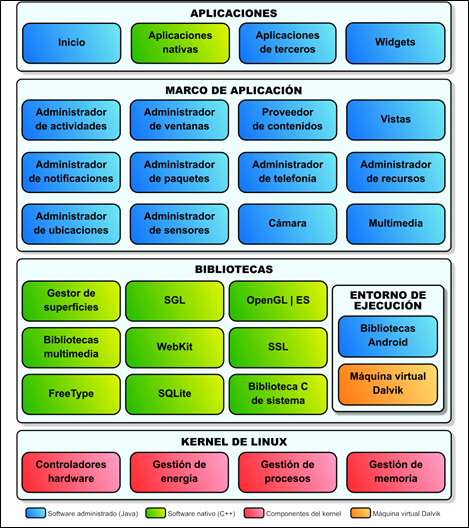
\includegraphics[scale=0.77]{images/Android-architecture}
\par\end{centering}

\caption{Diagrama de la arquitectura en capas empleada por Android\label{fig:Android-architecture}}
\end{figure}

\begin{itemize}
\item Kernel Linux: Android utiliza el núcleo de Linux como una capa de
abstracción de hardware para los dispositivos móviles. Esta capa contiene
los drivers necesarios para que cualquier componente de hardware pueda
ser utilizado mediante las llamadas correspondientes, sólo debe considerarse
al momento de incluir un nuevo componente de hardware que los fabricantes
hayan desarrollado los drivers correspondientes. Además del soporte
de drivers, la capa es responsable de proporcionar otros servicios
como la seguridad, el manejo de la memoria, procesos, etc. 
\item Entorno de ejecución de Android: como se ha adelantado previamente,
cada aplicación corre en su propio proceso Linux con su propia instancia
de la máquina virtual Dalvik, la cual interpreta un lenguaje ligeramente
diferente al tradicional bytecode de \ac{JVM}. A partir de la versión
5.0 de Android, Dalvik es reemplazada por \ac{ART} la cual logra
reducir el tiempo de ejecución del código Java hasta un 33\%. También
se incluye en el entorno un módulo de librerías nativas con la mayoría
de librerías disponibles en lenguaje Java. Estas bibliotecas, si bien
resultan diferentes a las ofrecidas por \ac{Java SE} y \ac{Java ME},
proveen prácticamente la misma funcionalidad. 
\item Bibliotecas: incluye un conjunto de bibliotecas nativas escritas en
lenguaje C y C++ usadas en varios componentes de Android que proporcionan
la mayor parte de las características de Android.
\item Marco o framework de Aplicaciones: este es el framework que proporciona
Android para el desarrollo de aplicaciones, servicios y otros componentes.
Todo el conjunto de funciones del sistema operativo y bibliotecas
nativas está disponible a través de este framework, cuya API esta
escrita en el lenguaje Java. El framework permite que los desarrolladores
tengan acceso a las mismas \ac{API} utilizadas por las aplicaciones
base del sistema. El foco principal del diseño de esta capa ha sido
simplificar la re-utilización de componentes: las aplicaciones pueden
publicar sus capacidades y otras pueden hacer uso de ellas (sujetas
a restricciones de seguridad), un mecanismo que permite a los usuarios
reemplazar fácilmente componentes. 
\item Aplicaciones: Este nivel contiene todas las aplicaciones de usuario,
tanto las incluidas por defecto en Android así como como aquellas
que el usuario vaya añadiendo posteriormente ya sean de terceros o
de su propio desarrollo. Todas estas aplicaciones utilizan los servicios,
las \ac{API} y bibliotecas de los niveles inferiores. Se brindará
una descripción más detallada en la siguiente sección.
\end{itemize}

\subsection{Aplicaciones Android \label{sec:Aplicaciones-Android}}

Además de las características técnicas, es importante resaltar que
la popularidad de Android ha crecido muy rápidamente desde su lanzamiento.
Esto se debe a la versatilidad que Android otorga a los dispositivos
a través de las aplicaciones, que permiten adaptarlos según las necesidades
de los usuarios. Android también permite que las aplicaciones se adapten
a las características del dispositivo (pantalla, sensores, etc.),
aprovechando las capacidades particulares de cada uno. 

Un aspecto clave del diseño de las aplicaciones en Android es que
éstas pueden reutilizar componentes de otras aplicaciones instaladas
en el dispositivo. Por ejemplo, si una aplicación desea tomar una
fotografía, es probable que ya exista una aplicación que cumpla esa
funcionalidad, entonces, la nueva aplicación puede utilizar la existente
sin necesidad de desarrollar una actividad propia para utilizar la
cámara, esta invocación se realiza de modo tal que sea transparente
para el usuario final.

El sistema Android provee cinco tipos de componentes básicos para
el desarrollo de aplicaciones: Activity, Service, Content Provider,
Broadcast Receiver e Intent. El componente \emph{Activity }representa
una pantalla simple que provee interfaz de usuario. Una aplicación
puede estar formada por una o mas actividades que trabajan en conjunto
y representan diferentes pantallas o vistas. 

Los\emph{ Content Providers} son los encargados de administrar la
información compartida por las aplicaciones. Las aplicaciones pueden
almacenar sus datos en el sistema de archivos, en una base de datos
SQLite, en la Web, o en cualquier otro lugar de acceso. A través del
\emph{content provider}, otras aplicaciones pueden consultar, o incluso
modificar estos datos. 

Las aplicaciones también pueden iniciar servicios que se ejecutan
en segundo plano para realizar operaciones que requieran gran cantidad
de tiempo, o interactúen con procesos remotos, por ejemplo la reproducción
de música en segundo plano o la descarga de datos mientras el usuario
interactúa con una aplicación diferente. 

El componente \emph{Intent} es un objeto de acción que facilita la
comunicación entre componentes. Un intent puede verse como un mensaje
entre componentes, por ejemplo, para iniciar una actividad o servicio,
o solicitar una acción. Por último, el componente \emph{Broadcast
Receiver} funciona como puerta de enlace a otros componentes, respondiendo
a los anuncios (Intents) originados por el sistema u otras aplicaciones,
por ejemplo, cuando la pantalla se apaga, la batería es baja, o al
capturar una fotografía. 


\section{Componentes de software\label{sec:Componentes-de-software}}

En el marco del desarrollo de software nos encontramos con la posibilidad
de reutilizar código previamente desarrollado, testeado y deployado
que cumple con una determinada funcionalidad, ahorrando tiempo y esfuerzo
al desarrollador. Estas piezas de códigos ya implementadas se distribuyen
como componentes de software que encapsulan a un conjunto de funciones
y datos relacionados. 

La re-utilización es uno de los objetivos principales al momento de
diseñar un componente de software de calidad para ser usado en diferentes
programas. La comunicación entre componentes se realiza a través de
interfaces. Cuando un componente ofrece servicios al resto del sistema,
el mismo proporciona una interfaz que especifica los servicios que
otros componentes pueden utilizar y la manera en que pueden hacerlo.
La interfaz puede verse como una firma del componente ya que el cliente
no necesita conocer el procesamiento interno del componente para utilizarlo,
condición que respeta el principio de encapsulamiento. Por otro lado,
cuando un componente necesita de otro para su funcionamiento, el mismo
establece las interfaces requeridas donde especifica los servicios
que necesita. De acuerdo al lenguaje de modelado \ac{UML}, las interfaces
proporcionadas por componentes son representadas con símbolos de lollipop
en el borde del componente y las interfaces requeridas por medio de
sockets abiertos en el borde externo, como se ilustra en la figura
\ref{fig:UML-component}. 

\begin{figure}
\begin{centering}
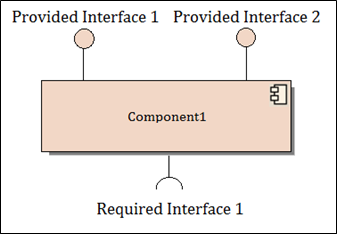
\includegraphics[scale=0.9]{images/UML-component}
\par\end{centering}

\caption{Componente UML con interfaces proveídas y requeridas.\label{fig:UML-component}}
\end{figure}


Otra de las características fundamentales de los componentes es su
capacidad de ser sustituidos tanto en tiempo de diseño como en tiempo
de ejecución, pudiendo ser reemplazados por actualizaciones u otras
alternativas sin romper el sistema en el que los componentes funcionan.
El reemplazo es posible si el componente sucesor provee al menos la
misma funcionalidad que el componente a reemplazar y si requiere a
lo sumo las mismas funciones que el componente inicial. 


\section{Atributos de calidad \label{sec:Atributos-de-calidad}}

Además de su interfaz y funcionalidad, los componentes de software
se caracterizan por un conjunto de propiedades que representan los
aspectos no-funcionales o de calidad de servicio, llamados propiedades
o atributos de calidad. Estas propiedades son características medibles
que utilizan los usuarios para juzgar su funcionamiento~\cite{McGraw2012}.
Algunos ejemplos de estas propiedades son: el tiempo de respuesta,
la disponibilidad, etc. 

Al diseñar un sistema de software no sólo se espera cumplir con los
objetivos de negocio sino también alcanzar un determinado grado de
calidad de software capaz de satisfacer al grupo de usuarios y/o diseñadores.
El diseño de la arquitectura de un sistema depende mayormente de los
atributos de calidad demandados por los stakeholders. Largos tiempos
de respuesta, caídas del sistema, interfaces confusas, no son características
deseables en un sistema, por lo que toda decisión respecto al diseño
de la arquitectura debe conducir al cumplimiento de ciertos atributos
de calidad al mismo tiempo que cumple con la funcionalidad requerida.

Estos atributos de calidad se pueden dividir en dos grupos en base
al momento en el cual son medidos. Un grupo incluye atributos cuantificados
durante el tiempo de diseño como la escalabilidad, modificabilidad,
etc. El segundo grupo incluye atributos cuantificables mientras el
sistema se ejecuta como usabilidad, seguridad, etc. Este trabajo se
enfoca en la predicción de propiedades dinámicas o en tiempo de ejecución.A
continuación se describen las dos propiedades consideradas en la evaluación
del enfoque. 


\subsection*{Tiempo de respuesta\label{subsec:Atributos-de-calidad-Performance}}

Se puede medir la calidad de un sistema a través de su desempeño (performance)
evaluando la efectividad del uso de los recursos disponibles en tiempo
de ejecución. Dependiendo el contexto, el desempeño puede medirse
a través de varias propiedades, como el tiempo de respuesta o la latencia.
El rendimiento de un sistema engloba, generalmente, el tiempo de los
eventos que se producen y que el sistema debe responder a ellos. Estos
eventos pueden ser muy variados tales como alarmas, mensajes, peticiones
a usuarios o procesamiento, pero básicamente se considera de todos
ellos el tiempo que tarda el sistema para responder al evento. La
complejidad para el manejo de estos eventos radica en su fuente, ya
que pueden provenir desde una solicitud de usuario, de otros sistemas
o desde el interior del propio sistema. 


\subsection*{Precisión\label{subsec:Atributos-de-calidad-Precisi=0000F3n}}

Cabe destacar que no existe una definición estándar sobre el significado
de precisión en un sistema, ya que se trata de una medida que evalúa
qué tan exacta es la respuesta de una función (operación) de un componente,
y cada función está ligada a resolver un problema o funcionalidad
particular. Por ejemplo, en un problema de detección de rostros, la
precisión puede medirse como la cantidad de rostros correctamente
detectados sobre los rostros totales presentes, y en un problema de
optimización puede significar el grado de cercanía del valor de la
solución encontrada respecto a la solución óptima.


\section{Aprendizaje de máquina \label{sec:Aprendizaje-de-maquina}}

El aprendizaje de máquina  o aprendizaje automático es una rama de
la inteligencia artificial cuyo objetivo es desarrollar técnicas que
permitan a las computadoras \emph{aprender} a partir de datos suministrados
en forma de ejemplo. El aprendizaje a partir de datos es la base para
comprender el proceso de aprendizaje de máquina ya que los datos son
la única herramienta de la que se dispone y conoce a ciencia cierta
sobre las características de un dominio cualquiera. El aprendizaje
de máquina puede entenderse haciendo una analogía con el aprendizaje
humano basado en la experiencia, en donde el hombre basa su conocimiento
en tres partes: \emph{i}) recuerdo, el hombre reconoce cuando ha sido
la última vez que estuvo en una determinada situación (dataset), \emph{ii})
adaptación, reconoce la última vez que se probó una acción (salida
producida) y \emph{iii}) generalización, reconoce si ha funcionado
o no esta acción (si fue correcta o no). El término generalización
refiere a la similitud entre diferentes situaciones de manera tal
que las opciones que han sido aplicadas en casos previos pueden ser
usadas en nuevos casos.

El aprendizaje de máquina, entonces, es un proceso para que las computadoras
modifiquen o adapten sus acciones (predictivas o de control) para
que sus resultados sean más precisos, precisión que refleja la proximidad
respecto a las acciones correctas. El aprendizaje de máquina reúne
ideas de neurociencia, biología, estadística, matemática y física,
para generar técnicas y hacer que la computadora aprenda. Un área
importante relacionada con el aprendizaje de máquina es la minería
de datos, el proceso de extraer información útil de un conjunto de
datos masivos por medio de algoritmos eficientes. 

Si se define el aprendizaje de máquina como la mejora de tareas a
través de la experiencia, surge el cuestionamiento de como la computadora
puede saber si está aprendiendo mejor o de qué forma podría mejorar
ese aprendizaje. De aquí, surgen diferentes tipos de técnicas o algoritmos
de aprendizaje. Por ejemplo, se le puede indicar a un algoritmo la
respuesta correcta para un problema, así, la próxima vez que se aplique
su desempeño será mejor. También, podría indicarse un conjunto de
respuestas correctas para que el algoritmo \emph{adivine} la forma
de obtener estas respuestas para otros problemas (generalización).
Alternativamente, se puede indicar si la respuesta obtenida es correcta
o no sin señalar la respuesta real, que el algoritmo debería ser capaz
de encontrar. Una variante podría ser asignarle un puntaje a la respuesta
obtenida por el algoritmo que indique cuán correcta resulta ser. 

Estas diferentes alternativas proveen una forma de clasificar las
diferentes métodos de aprendizaje que será detallada en la siguiente
sección. Cabe destacar que por más que existan distintos tipos de
aprendizaje, todos los métodos comparten el mismo objetivo de generalización:
la técnica debe producir salidas sensibles para datos de entrada que
no fueron encontrados durante el aprendizaje, teniendo en cuenta también
que el algoritmo debe lidiar con ruido en los datos, es decir, imprecisión
en los valores que es inherente a la medición de cualquier proceso
real. 


\subsection{Clasificación de las técnicas de aprendizaje}



El modo de aprendizaje que una técnica particular puede realizar queda
determinado por la naturaleza de los datos de entrada, es decir, los
datos de entrenamiento (\emph{dataset}). Básicamente las técnicas
de aprendizaje se clasifican en tres grandes grupos: aprendizaje supervisado,
no supervisado, y por refuerzo.

El aprendizaje supervisado utiliza un conjunto de datos basado en
dos pares de objetos: los datos de entrada o conjunto de ejemplos
del dominio y las respuestas correctas (\emph{targets}) para una propiedad
determinada . A través de las respuestas correctas provistas y basado
en el conjunto de datos la técnica de aprendizaje generaliza el comportamiento
para responder a todas las posibles entradas. Este modo de aprendizaje,
entonces, es un proceso que se realiza mediante un entrenamiento controlado
por un agente externo que determina la respuesta que debería generar
la técnica a partir de una entrada determinada. 

Dentro del aprendizaje supervisado, las técnicas pueden separarse
en dos grupos de acuerdo a la naturaleza de la propiedad o respuesta. 
\begin{description}
\item [{Clasificación}] Consiste en asignar a cada ejemplo una etiqueta
o clase a la que pertenece basado en el entrenamiento de ejemplares
de cada clase. Los datos de entrenamiento son instancias que pertenecen
a una única clase y el conjunto de clases cubre todas las salidas
posibles, por eso se considera al proceso de clasificación como un
proceso discreto. El algoritmo de clasificación tiene como objetivo
encontrar umbrales de decisión que sirvan para identificar las diferentes
clases.
\item [{Regresión}] El proceso de regresión predice valores numéricos de
atributos a partir de funciones matemáticas polinomiales que describan
o se ajusten lo más posible a todos los puntos del dominio, es decir,
todos los valores del conjunto de entrenamiento correspondientes a
la propiedad que se quiere predecir. Generalmente, se considera un
problema de aproximación de función o interpolación al encontrar un
valor numérico entre los valores conocidos. Por lo tanto, el eje primordial
del proceso de regresión es encontrar la función que mejor represente
al conjunto de puntos, ya que funciones con distintos grados de polinomios
producen diferentes efectos.
\end{description}
En el aprendizaje no supervisado, la máquina simplemente recibe los
datos de entrada sin etiquetas o respuestas correctas como en el método
supervisado, ni valores de recompensa desde el ambiente. Aun así,
es posible desarrollar un framework formal para llevar a cabo aprendizaje
no supervisado basado en la noción de que el objetivo es construir
una representación de la entrada que puede ser usada para tomar decisiones,
predecir futuras entradas, comunicar eficientemente entradas para
otras máquinas, entre otras posibilidades. 

El aprendizaje no supervisado puede entenderse como la búsqueda de
patrones en los datos independientemente del ruido presente en los
mismos. Por ejemplo, las técnicas de agrupamiento (clustering) son
técnicas de aprendizaje no supervisado que agrupan un conjunto de
objetos de modo tal que los objetos pertenecientes a un mismo grupo
(\emph{cluster}) comparten algún tipo de similitud entre ellos, de
igual sentido que se diferencian con los objetos de otro grupo. A
diferencia del proceso de clasificación, los grupos o clases no son
conocidos fehacientemente antes del entrenamiento, un claro método
de aprendizaje no supervisado. 

Por ultimo, el aprendizaje por refuerzo se basa en la idea de no disponer
de ejemplos completos del comportamiento deseado por el algoritmo,
es decir, no indicar durante el entrenamiento exactamente la salida
que se desea proporcione el clasificador ante una determinada entrada,
sólo se le indica si la salida obtenida se ajusta a la deseada y en
función a ello se re configuran los pasos. 


\subsection{Técnicas contempladas\label{subsec:Funciones-contempladas}}

El foco principal del trabajo es el desarrollo de un enfoque para
predecir propiedades no-funcionales de componentes de software en
ejecución, como el tiempo de respuesta, precisión de las respuestas,
entre otros. Estas propiedades son valores continuos, motivo por el
cual se entrenan y evalúan técnicas de regresión para su predicción.
Las técnicas utilizadas se describen a continuación. 




\subsubsection{Regresión Lineal\label{sub:Regresi=0000F3n-Lineal}}

La regresión es la predicción de un valor desconocido a través del
cálculo de una función matemática a partir de los valores conocidos.
Si se considera esta función como una función lineal, la salida será
la suma de cada valor conocido multiplicado por una constante, lo
cual define una línea recta (plano en 3D o hiperplano en dimensiones
mayores) que circundan los puntos, como puede observarse en la Figura
\ref{fig:regression-lineal}. 

\begin{figure}
\begin{centering}
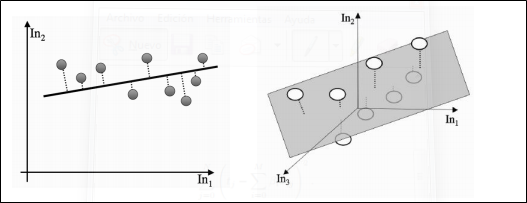
\includegraphics[scale=0.85]{images/regression-lineal}
\par\end{centering}

\caption{Regresiones lineales en dos y tres dimensiones.. \label{fig:regression-lineal}}
\end{figure}


Para encontrar la recta (función lineal) que mejor se \emph{ajusta}
a los datos, se intenta minimizar la distancia entre cada punto y
dicha recta. Esta distancia se mide a través de una línea auxiliar
que atraviesa el punto y tope con la función. Luego, se intentará
minimizar la función de error que que se calcula como la suma de las
distancias. Si se minimiza la suma de los cuadrados de las distancias,
se obtiene la minimización más común llamada optimización de mínimos
cuadrados. 

La minimización de este error, para ajustar la función lineal, puede
realizarse con distintas técnicas de regresión lineal, como \emph{ridge-regression
}y \emph{gradiente estocástico descendiente}. La primera aplica una
penalización (\emph{ridge}) a cada constante. La segunda, aplica un
diferencial sobre la función obteniendo el gradiente el cual por definición,
es la dirección en la que incrementa o disminuye en mayor medida.
Ya que el propósito del aprendizaje es minimizar el error de predicción,
se debe seguir la función en dirección del gradiente negativo en la
cual la función disminuye. 


\subsubsection{Red neuronal}

La técnica de red neuronal presenta un modelo matemático sobre el
comportamiento de una neurona.El mismo representa una célula nerviosa
como \emph{i}) un conjunto de entradas valoradas (w) que corresponde
a las sinapsis, \emph{ii}) un sumador que une las señales entrantes
y \emph{iii}) una función de activación (inicialmente una función
umbral) que decide sobre la activación de la célula en base a las
entradas actuales. 

\begin{figure}
\begin{centering}
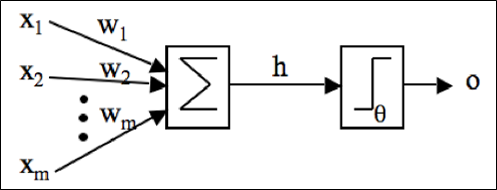
\includegraphics[scale=0.85]{images/McCulloch-Pitts}
\par\end{centering}

\caption{Modelo matemático neuronal . \label{fig:McCulloch-Pitts}}
\end{figure}


Como puede observarse en la figura \ref{fig:McCulloch-Pitts}, el
modelo neuronales un dispositivo límite binario, las entradas son
multiplicadas por los pesos y sumando sus valores; si la suma es mayor
a un determinado umbral (produce salida 1) la célula se activa, de
lo contrario (produce salida 0) se mantiene desactivada.

El perceptron es una colección de neuronas con un conjunto de entradas
y pesos que unen las neuronas con dichas entradas. Las neuronas del
Perceptron son completamente independientes entre sí, el estado de
una neurona no infiere sobre las demás compartiendo sólo las entradas.

La esencia del aprendizaje de la red neuronal perceptron está centrada
en los valores de pesos. La red debe ser entrenada para que los pesos
se adapten y generen las respuestas correctas (\emph{targets}).

El entrenamiento de \ac{MLP} consiste en dos partes, primero se obtienen
las salidas con las entradas brindadas y los pesos actuales (\emph{forwards}),
y luego se actualizan los pesos considerando el error como la diferencia
entre el valor obtenido y el real (propagación hacia atrás del error
- \emph{backwards}). 

\begin{figure}
\begin{centering}
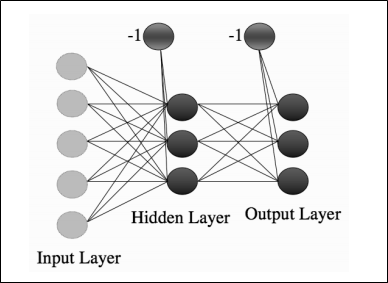
\includegraphics[scale=0.85]{images/Perceptron-multilayer}
\par\end{centering}

\caption{Red perceptrón multicapa\label{fig:perceptron-neural-network-multilayer}}
\end{figure}



\subsubsection{K-means clusterer}

El algoritmo K - means aplica clustering sobre los datos de entrenamiento
y recibe un parámetro \emph{K} para dividir estos datos en \emph{K}
categorías. El algoritmo intenta localizar k centros en el espacio
de entrada de modo tal que estos centros estén, como su nombre lo
indica, en el centro de una categoría (\emph{cluster}). La dificultad
se presenta ya que al desconocer la categorización de estos grupos,
resulta aún más difícil determinar la localización de cada centro. 

El objetivo de determinar estos centros, en principio, a causa de
incertidumbre total se posicionan los centros de forma aleatoria en
el espacio de entrada. Una vez distinguidos los clusters, se determinan
los puntos que pertenecen al mismo a través del cálculo de la distancia
entre el punto y todos los centros localizados, asignándose entonces,
al cluster cuyo centro sea el más cercano. Finalmente, para cada centro
se actualiza su ubicación utilizando la media antes definida. Estos
pasos se realizan de forma incremental hasta que los centros dejan
de modificar su ubicación. 

Ya que este algoritmo sin duda es un método de clasificación y no
de regresión, se considera importante resaltar la adaptación del mismo
para utilizarlo con este fin. Así, una vez realizada la clasificación
del punto que se quiere predecir, se realizará la predicción calculando
el promedio de los valores de la propiedad a predecir de los otros
puntos que están en el cluster. 


\subsubsection{Maquina de vector de soporte}

La técnica de máquina de vector soporte \ac{SVM}. es un método propiamente
relacionado con problemas de clasificación y regresión. Dado un conjunto
de ejemplos de entrenamiento (dataset) se pueden etiquetar las clases
y entrenar un SVM para construir un modelo que prediga la propiedad
de un nuevo dataset. Intuitivamente, un SVM es un modelo que representa
a los puntos de muestra en el espacio, separando las clases en dos
espacios lo más amplios posibles mediante un hiperplano de separación.
Analíticamente, se toma la distancia existente entre la línea y el
primer punto interceptado (en dirección perpendicular), si se ubica
una ‘zona desierta’ alrededor de la línea, ningún punto ubicado en
dicha zona puede ser clasificado ya que se encuentra demasiado cerca
de la línea. El radio máximo que puede tener esta región es llamado
margen, señalado como M y los puntos de cada clase más cercanos a
la línea de clasificación se denominan vectores de soporte

\begin{figure}
\begin{centering}
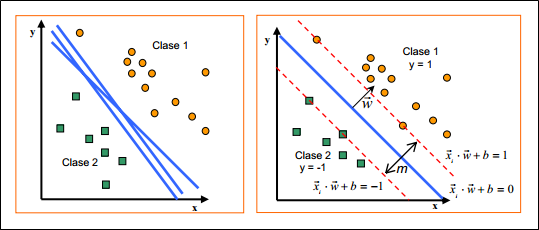
\includegraphics[scale=0.9]{images/SVM-metology}
\par\end{centering}

\caption{Metodología de operación del algoritmo SVM\label{fig:SVM-metology}}
\end{figure}



\subsection{Evaluación de modelos}

Una vez entrenado un modelo de predicción con una técnica, la evaluación
del modelo es importante para medir el nivel de acierto de las predicciones.
Esta evaluación consiste en probar el modelo con un conjunto de datos
de prueba y medir el error u otras métricas sobre los resultados.
Estas métricas de evaluación permite comparar el desempeño de modelos
entrenados con diferentes técnicas. 

Existen distintas formas para llevar a cabo esta evaluación. La mas
simple consiste en usar como datos de prueba el mismo conjunto de
datos utilizado para el entrenamiento de los modelos. Otro método
consiste en separar los datos del problema entre datos de entrenamiento
y datos de prueba. Por ultimo, también se puede validar el modelo
de forma cruzada. 

La validación cruzada (cross-validation) es una técnica utilizada
para evaluar los resultados de un análisis estadístico y garantizar
que son independientes de la partición entre datos de entrenamiento
y prueba. Consiste en repetir y calcular la media aritmética obtenida
de las medidas de evaluación sobre diferentes particiones. Por ejemplo,
si consideramos diez subconjuntos para validación, los datos de entrada
se dividen en diez partes, donde una se reserva para las pruebas y
las otras nueve para el entrenamiento. Este proceso se repite diez
veces y se calcula el promedio de las métricas de evaluación. Esto
ayuda a determinar el nivel al que un modelo se podría generalizar
para nuevos conjuntos de datos. 

El presente trabajo contempla las siguientes métricas de evaluación
para los modelos de regresión: 
\begin{itemize}
\item CC (Coeficiente de correlación de Pearson): el coeficiente de correlación
de Pearson es un índice que puede utilizarse para medir el grado de
relación de dos variables siempre y cuando ambas sean cuantitativas.
En el presente trabajo se considera la correlación entre las variables
del dataset con respecto a la propiedad a predecir.
\item RMSE (Root Mean Absolute Error): el \ac{RMSE} representa la raiz
cuadrática del promedio de la distancia euclídea entre el valor de
la propiedad obtenida por la técnica y el valor real. 
\end{itemize}

\subsection{Ajuste del modelo: Overfitting y Underfitting\label{sub:Ajuste-del-modelo:}}

Cuando se genera (o entrena) un modelo de predicción, su desempeño
es incierto hasta su evaluación o aplicación. En algunas ocasiones,
la calidad del modelo es pobre generando respuestas imprecisas, de
modo tal que se le deben aplicar acciones correctivas comprendiendo
cómo se comporta y ajusta el modelo. 

Los modelos pueden presentar dos problemas indeseables: \emph{overfitting}
y \emph{underfitting}. El \emph{overfitting }describe una función
que se ajusta estrechamente a los datos de entrenamiento. El modelo
aprendió los detalles y el ruido en los datos impactando negativamente
en el desempeño del modelo. Este efecto es causado porque el ruido
o las fluctuaciones aleatorias en los datos de entrada fueron usados
para el aprendizaje. 

Por otro lado, los modelos pueden presentar problemas de \emph{underfitting},
cuando no interpretan bien los datos de entrenamiento, por lo que
son incapaces de generalizar correctamente nuevos datos. Este efecto
es causado porque la función o técnica elegida no es el indicada para
representar el comportamiento de los datos. El efecto underfitting
se caracteriza por sobre generalizar los datos. La incorporación de
nuevos datos al conjunto de entrenamiento podría solucionar o apaciguar
este efecto. 

El modelo deseado, sin dudas, sería aquel que se encuentre en un punto
de equilibrio entre un problema y otro, aunque este equilibrio es
muy difícil de alcanzar en la práctica. La Figura \ref{fig:under-overfitting}
presenta tres modelos de regresión para un mismo grupo de datos que
permiten interpretar gráficamente los problemas de underfitting y
overfitting.

\begin{figure}
\begin{centering}
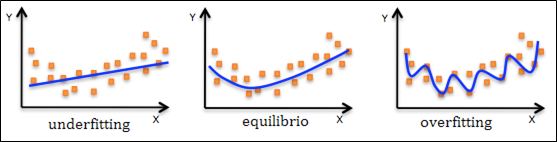
\includegraphics[scale=0.85]{images/under-overfitting}
\par\end{centering}

\caption{Contraste entre distintos efectos del modelo sobre los datos de entrenamiento.\label{fig:under-overfitting}}
\end{figure}




  
